% !Mode:: "TeX:UTF-8"
\documentclass{apmcmthesis}

\usepackage{url}
\usepackage{subcaption}
\usepackage{float}
\usepackage{lastpage}
\usepackage{graphicx}
\usepackage{amsmath}
\usepackage{caption}
\usepackage{tikz}
\usetikzlibrary{arrows.meta, positioning}

\tikzstyle{block} = [rectangle, draw, rounded corners, align=center, minimum height=2em, minimum width=3cm]

%%%%%%%%%%%%填写相关信息%%%%%%%%%%%%%%%%%%%%%%%%%%
\tihao{A}                            %选题
\baominghao{apmcm24207116}           %参赛编号

\begin{document}

\pagestyle{frontmatterstyle}

\begin{abstract}
    Underwater images often suffer from significant degradation due to the complex imaging environment, including color distortion, low brightness, and blurriness.

    This paper introduces a multi-faceted enhancement approach that addresses both single and multiple degradation types. For individual degradation factors, we design specific enhancement methods: utilizing the gray world assumption for precise color correction, applying histogram equalization to enhance brightness, and implementing unsharp masking to reduce blurriness. These traditional methods are optimized to work synergistically, ensuring targeted precision for each degradation type.
    
    To manage complex underwater environments with multiple overlapping degradations, we develop an advanced deep learning model based on an improved U-Net architecture. This model integrates a pre-trained ResNet encoder for deep feature extraction and incorporates Squeeze-and-Excitation (SE) blocks to enhance feature recalibration. Attention mechanisms are further integrated to focus on critical image areas requiring enhancement. The model is trained on a comprehensive dataset of degraded and enhanced underwater images, ensuring high adaptability and robustness across various scenarios.
    
    Experimental evaluations using both subjective visual assessments and objective metrics, including Peak Signal-to-Noise Ratio (PSNR), Structural Similarity Index Measure (SSIM), Underwater Color Image Quality Evaluation (UCIQE), and Underwater Image Quality Measure (UIQM), demonstrate that our proposed strategies significantly improve image quality. The deep learning model outperforms existing methods in restoring color fidelity, enhancing brightness, and sharpening details while maintaining computational efficiency.
    
    In conclusion, the proposed enhancement strategy effectively mitigates underwater image degradation by integrating targeted traditional methods with an advanced deep learning framework. This hybrid approach achieves substantial improvements in both subjective and objective evaluations, facilitating more accurate and reliable underwater visual analyses.
\keywords{Underwater Image Enhancement \quad Image Degradation Model \quad White Balance Correction \quad Deep Learning \quad Attention Mechanism}
\end{abstract}

\newpage
%目录
\tableofcontents

\newpage
\pagestyle{mainmatterstyle}
\setcounter{page}{1}

\section{Introduction}

\subsection{Background and Motivation}
With the advancement of ocean exploration, high-quality underwater images have become crucial for marine research, resource exploration, and archaeological studies. However, the complex underwater environment significantly degrades image quality through various optical phenomena, including light absorption, scattering, and diffraction. These degradation effects manifest as color distortion, low brightness, poor contrast, and blurriness, severely hindering subsequent visual analysis tasks.

\subsection{Previous Solutions and Limitations}
Traditional approaches to underwater image enhancement can be categorized into two main streams: physical model-based methods and non-physical model-based methods. Physical models attempt to reverse the degradation process by estimating environmental parameters, often utilizing priors such as dark channel or dehazing assumptions. \cite{cong2023pugan} While theoretically sound, these methods struggle with complex real-world scenarios. Non-physical approaches, including histogram equalization and color correction, offer simple and efficient solutions but typically address only specific degradation types.

\subsection{Deep Learning Approaches}
Recent years have witnessed the emergence of deep learning techniques in underwater image enhancement. Despite their potential for end-to-end enhancement, conventional CNNs face inherent limitations. Their uniform convolution kernels struggle to capture varying attenuation patterns across different channels and regions, while their focus on local features limits their ability to model global dependencies. \cite{peng2023u} Although hybrid architectures combining CNNs with Transformers and attention mechanisms show promise, they require substantial high-quality training data, which remains scarce in underwater scenarios.

\subsection{Our Contributions}
This paper presents a comprehensive enhancement framework that leverages both traditional and deep learning methods. We first develop targeted solutions for specific degradation types, then propose an attention-enhanced neural network for complex scenarios. Our approach achieves robust performance while maintaining computational efficiency, addressing the practical challenges of underwater image enhancement.

\begin{itemize}
    \item \textbf{Rapid Enhancement for Single Degradations:} Utilizing traditional image processing techniques such as white balance correction based on the gray world assumption, histogram equalization for brightness enhancement, and unsharp masking for deblurring to quickly and effectively improve image quality.
    \item \textbf{Improved Deep Learning Model:} Designing a U-Net-based \cite{ronneberger2015u} underwater image enhancement model that incorporates a pre-trained ResNet encoder \cite{he2016deep} for its rich feature representation capabilities and integrates attention mechanisms (SE modules) to emphasize important features, thereby improving enhancement performance.
    \item \textbf{Lightweight and Efficient Training:} Reducing model complexity and computational requirements through model pruning, loss function optimization, and mixed-precision training, enhancing training and inference efficiency.
    \item \textbf{Data Augmentation and Simulation:} Addressing the lack of paired datasets by using images enhanced with traditional methods as training targets for deep learning models and employing data augmentation techniques to improve model generalization capabilities.
\end{itemize}

Through these strategies, this paper achieves comprehensive enhancement of underwater images, enabling rapid processing of single degradation types and leveraging deep learning models to handle complex degradation scenarios, thereby improving both visual quality and objective evaluation metrics.

\section{Problem Description and Analysis}
Before tackling the complex task of underwater image enhancement, it is essential to comprehend the underlying mechanisms and manifestations of image degradation. We adopt a hierarchical and progressive research approach, transitioning from single-degradation scenarios to complex, multi-degradation environments, and from traditional methods to deep learning techniques to build a comprehensive solution.

Initially, we establish a reliable image classification system that accurately identifies degradation types through multidimensional feature analysis. This involves basic color histogram analysis and feature extraction across multiple color spaces (RGB, LAB, HSV), combined with frequency domain analysis and edge detection. Such multi-perspective analysis ensures precise classification, laying the groundwork for targeted enhancement processes.

With accurate classification, we explore the degradation mechanisms by constructing a physical model of underwater image degradation. This model describes light attenuation and scattering in water, accounting for wavelength-dependent absorption (causing color distortion), scattering effects (causing blurriness), and depth-dependent light intensity attenuation (causing low brightness). Through theoretical analysis and experimental validation, we elucidate the interrelationships among various degradation factors and their combined impact on image quality.

For single types of degradation, we develop enhancement algorithms grounded in physical models. For instance, to mitigate color distortion, we introduce an improved white balance algorithm that analyzes the statistical properties of each color channel, combining color temperature adjustment with gain control to achieve natural color restoration. This method is computationally efficient and physically interpretable, facilitating parameter tuning and optimization.

However, real-world underwater scenarios often involve overlapping degradation effects, necessitating comprehensive enhancement methods. To address this, we design a deep learning-based enhancement model built on an improved U-Net architecture with integrated attention mechanisms. This model learns to identify and correct multiple degradation types simultaneously through large-scale data training, achieving end-to-end image enhancement. Additionally, we implement a multi-scale feature fusion strategy and a hybrid loss function to ensure high visual quality in the enhanced images.

\section{Model Assumptions}
To establish a reliable underwater image enhancement system, we make the following assumptions based on the characteristics of underwater imaging and the requirements of image processing:
\begin{itemize}
    \item 1. Assume that the degradation of underwater images is mainly influenced by light absorption and scattering, with other factors (e.g., water temperature, pressure) negligible.
    \item 2. Assume that the water medium is uniformly distributed in local regions, meaning that at the same depth plane, properties like water turbidity and suspended particle density remain consistent.
    \item 3. Assume that the attenuation coefficients of light with different wavelengths in water are stable. Red light attenuates the fastest, followed by green and blue light, with attenuation rates following an exponential law.
    \item 4. Assume that the degree of image degradation is monotonically related to water depth, where increasing depth results in stronger attenuation, scattering, and blurring effects.
    \item 5. Assume that the deep learning model can effectively learn statistical properties of underwater scenes during training, and these properties apply to test images.
    \item 6. Assume that single-scene degradations (e.g., color cast) can be independently addressed by corresponding physical models, while multiple degradations can be comprehensively handled through combined models or deep learning methods.
    \item 7. Assume that the image enhancement process does not introduce new degradation, ensuring that the quality of the enhanced image is never inferior to the original.
\end{itemize}

\section{Model Development}

\subsection{Problem 1: Underwater Image Degradation Identification Model}

\subsubsection{Overview}

Underwater images often suffer from degradation phenomena such as color cast, insufficient brightness, and blurriness due to light absorption and scattering in water. To effectively identify these degradation types, we established a comprehensive underwater image degradation identification model to analyze and evaluate features such as color, brightness, and sharpness.

\subsubsection{Terminology and Notation}
Before describing the model, we define the related terminology and notation:

\begin{align*}
    &I(x, y): &&\text{The color pixel value at position } (x, y) \text{ in the image, including red, green,} \\
    &&&\text{and blue channels, } I = [I_R, I_G, I_B]. \\
    &\mu_c: &&\text{The average value of pixels in color channel } c, \text{ where } c \in \{R, G, B\}. \\
    &\sigma_c: &&\text{The standard deviation of pixels in color channel } c. \\
    &\Delta_{\text{gray}}: &&\text{Gray-world deviation, measuring the dispersion of RGB channel averages.} \\
    &L(x, y): &&\text{The grayscale pixel value at position } (x, y). \\
    &\nabla^2 L: &&\text{The Laplacian operator response of the grayscale image.} \\
    &\mathcal{F}(L): &&\text{The Fourier transform of the grayscale image } L. \\
    &E_{\text{high}}: &&\text{The high-frequency energy ratio, quantifying high-frequency components} \\
    &&&\text{in the image.} \\
    &\text{Skewness}: &&\text{The skewness of grayscale pixel values, reflecting the asymmetry of} \\
    &&&\text{brightness distribution.}
\end{align*}


\subsubsection{Model Development}

The degradation identification model consists of three components: color cast detection, low-light detection, and blur detection.

\paragraph{1. Color Cast Detection}
Color cast refers to an overall tendency towards a specific color in the image, typically caused by wavelength-dependent light absorption underwater. The following methods are used for detection:

(1) Gray-World Assumption  
Based on the Gray-World Assumption, the average reflectance in natural scenes should be equal across all color channels. Compute the RGB channel averages $\mu_R$, $\mu_G$, $\mu_B$, and calculate their deviation:  
\[
\Delta_{\text{gray}} = \frac{1}{3} \left( |\mu_R - \mu_G| + |\mu_G - \mu_B| + |\mu_B - \mu_R| \right)
\]  
If $\Delta_{\text{gray}}$ exceeds the threshold $T_{\text{gray}}$, a color cast is detected.

(2) LAB Color Space Analysis  
Convert the image from RGB to LAB color space, where $a$ and $b$ channels represent color components, and $l$ represents brightness. For images without color cast, the average values of $a$ and $b$ channels should be close to 128. Compute the color deviation:  
\[
\Delta_{\text{lab}} = \sqrt{ (\mu_a - 128)^2 + (\mu_b - 128)^2 }
\]  
where $\mu_a$ and $\mu_b$ are the average values of $a$ and $b$ channels, respectively. If $\Delta_{\text{lab}}$ exceeds the threshold $T_{\text{lab}}$, a color cast is detected.

\begin{figure}[!ht]
    \centering
    \includegraphics[width=\textwidth]{figures/image_004.png}
    \caption{Color Cast Detection Example}
    \label{fig:example_1}
\end{figure}

(3) HSV Color Space Analysis  
In HSV color space, saturation $S$ represents color purity. Compute the standard deviation of the $S$ channel:  
\[
\Delta_{\text{hsv}} = \sigma_S
\]  
A small $\Delta_{\text{hsv}}$ indicates uniform color distribution, suggesting a potential color cast.

\paragraph{2. Low-Light Detection}
Low-light images are typically characterized by low overall brightness and weak contrast. Detection methods include:

(1) Grayscale Mean and Standard Deviation  
Convert the color image to a grayscale image $L(x, y)$, and compute the mean $\mu_L$ and standard deviation $\sigma_L$:  
\[
\mu_L = \frac{1}{MN} \sum_{x=1}^{M} \sum_{y=1}^{N} L(x, y)
\]
\[
\sigma_L = \sqrt{ \frac{1}{MN} \sum_{x=1}^{M} \sum_{y=1}^{N} \left( L(x, y) - \mu_L \right)^2 }
\]
where $M$ and $N$ are the image width and height.

(2) Brightness Skewness  
Compute the skewness of the grayscale image to measure brightness asymmetry:  
\[
\text{Skewness} = \frac{ \frac{1}{MN} \sum\limits_{x=1}^{M} \sum\limits_{y=1}^{N} \left( L(x, y) - \mu_L \right)^3 }{ \sigma_L^3 }
\]
A negative skewness indicates left-skewed brightness distribution, suggesting a low-light image.

(3) Dark Pixel Ratio  
Set a brightness threshold $T_{\text{dark}}$ and compute the ratio of pixels with brightness below $T_{\text{dark}}$:  
\[
R_{\text{dark}} = \frac{ \sum\limits_{x=1}^{M} \sum\limits_{y=1}^{N} \delta \left( L(x, y) < T_{\text{dark}} \right) }{ MN }
\]
where $\delta$ is an indicator function that equals 1 if the condition is met, otherwise 0. If $R_{\text{dark}}$ exceeds the threshold, the image is classified as low-light.

\begin{figure}[!ht]
    \centering
    \includegraphics[width=\textwidth]{figures/image_009_low_light.png}
    \caption{Brightness distribution analysis of the image. The horizontal axis represents pixel brightness values (0-255), and the vertical axis denotes the frequency of pixels for each brightness level. The histogram shows a significant concentration of pixels in the lower brightness range (peak around 50), indicating low-light conditions in the image. The red dashed line marks the low-light threshold (approximately 90), serving as a reference for identifying and enhancing low-light regions.}
\end{figure}

\paragraph{3. Blur Detection}
Blurry images typically lack clear details and edges. Detection methods include:

(1) Laplacian Variance  
Compute the Laplacian operator response $\nabla^2 L$ of the grayscale image, then calculate its variance $\sigma_{\nabla L}^2$:  
\[
\nabla^2 L = \frac{\partial^2 L}{\partial x^2} + \frac{\partial^2 L}{\partial y^2 }
\]
\[
\sigma_{\nabla L}^2 = \frac{1}{MN} \sum_{x=1}^{M} \sum_{y=1}^{N} \left( \nabla^2 L(x, y) - \mu_{\nabla L} \right)^2
\]
where $\mu_{\nabla L}$ is the mean of $\nabla^2 L$. A lower variance indicates weaker edge strength, suggesting blurriness.

(2) High-Frequency Energy Ratio  
Perform Fourier transform on the grayscale image to obtain the spectrum $\mathcal{F}(L)$, and calculate the high-frequency energy ratio $E_{\text{high}}$:  
\[
E_{\text{high}} = \frac{ \sum\limits_{ (u, v) \in \text{High} } |\mathcal{F}(L)(u, v)|^2 }{ \sum\limits_{u=1}^{M} \sum\limits_{v=1}^{N} |\mathcal{F}(L)(u, v)|^2 }
\]
where "High" denotes the high-frequency region. A lower $E_{\text{high}}$ indicates potential blurriness.

\begin{figure}[!ht]
    \centering
    \includegraphics[width=\textwidth]{figures/image_009_blur.png}
    \caption{Edge detection analysis of a blurred underwater image. The left panel shows the original blurred image captured underwater. The middle panel illustrates edge detection using the Canny algorithm, highlighting primary structures with sparse edges. The right panel demonstrates edge enhancement via the Laplacian operator, revealing more detailed edges but introducing additional noise. This comparison highlights the trade-off between edge clarity and noise sensitivity in blur detection methods.}
    \label{fig:example_3}
\end{figure}

\subsubsection{Comprehensive Judgment and Classification}
\paragraph{1. Weighted Score Calculation}  
Weights are assigned to features of each degradation type, and the weighted scores are calculated as follows:

Color distortion score $S_{\text{color}}$:
\[
S_{\text{color}} = w_1 \frac{\Delta_{\text{gray}}}{T_{\text{gray}}} + w_2 \frac{\Delta_{\text{lab}}}{T_{\text{lab}}} + w_3 \frac{\Delta_{\text{hsv}}}{T_{\text{hsv}}}
\]

Low illumination score $S_{\text{light}}$:
\[
S_{\text{light}} = w_4 \left( 1 - \frac{\mu_L}{T_{\mu}} \right) + w_5 \frac{R_{\text{dark}}}{T_{\text{dark ratio}}} + w_6 \left( 1 - \frac{\text{Skewness}}{T_{\text{skewness}}} \right)
\]

Blur score $S_{\text{blur}}$:
\[
S_{\text{blur}} = w_7 \left( 1 - \frac{\sigma_{\nabla L}}{T_{\sigma}} \right) + w_8 \left( 1 - \frac{E_{\text{high}}}{T_{\text{high}}} \right)
\]

Here, $w_i$ represents feature weights, and $T$ is the corresponding threshold.

\paragraph{2. Classification Decision}  
A scoring threshold $S_{\text{th}}$ is set, and classification is performed based on the scores:
\begin{itemize}
    \item If $S_{\text{color}} > S_{\text{th}}$, the image is classified as color-distorted.
    \item If $S_{\text{light}} > S_{\text{th}}$, the image is classified as low illumination.
    \item If $S_{\text{blur}} > S_{\text{th}}$, the image is classified as blurry.
    \item If multiple scores of an image exceed the threshold, it is identified as having multiple types of degradation.
\end{itemize}

\subsection{Problem 2: Physical Model of Underwater Image Degradation}
\subsubsection{Principles of Underwater Imaging}
Underwater imaging is affected by light absorption and scattering, leading to quality degradation. The classical underwater imaging model describes the physical process of light propagation and imaging in water, expressed as:

\[
I(x) = J(x) t(x) + B \left( 1 - t(x) \right)
\]

where:
\begin{itemize}
    \item $I(x)$: observed pixel value at position $x$,
    \item $J(x)$: scene radiance without degradation,
    \item $t(x)$: transmission rate, representing energy attenuation of light passing through water,
    \item $B$: background light, representing environmental light contribution caused by scattering.
\end{itemize}

The transmission rate $t(x)$ is described by an exponential attenuation model:

\[
t(x) = e^{-\beta d(x)}
\]

where $\beta$ is the medium attenuation coefficient, and $d(x)$ is the scene depth.

\subsubsection{Modeling of Degradation Types}
\paragraph{1. Color Attenuation (Color Distortion)}  
Due to water's different absorption rates for various wavelengths, red light attenuates the fastest, followed by green and blue. For each color channel $c$, the transmission rate is:

\[
t_c(x) = e^{-\beta_c d(x)}
\]

where $\beta_c$ is the attenuation coefficient for channel $c$, and $\beta_R > \beta_G > \beta_B$. As a result, observed image colors are distorted, causing color shifts.

\paragraph{2. Brightness Attenuation (Low Illumination)}  
Water absorption leads to exponential attenuation of overall light intensity with depth:

\[
L(x) = L_0 e^{-\eta d(x)}
\]

where $L_0$ is the incident light intensity, and $\eta$ is the combined attenuation coefficient. As $d(x)$ increases, $L(x)$ significantly decreases, resulting in low illumination.

\paragraph{3. Forward Scattering Blur}  
Suspended particles in water scatter light, causing image blur, which can be modeled using convolution:

\[
I_{\text{blur}}(x) = \left[ J(x) * h(x) \right] t(x) + B \left( 1 - t(x) \right)
\]

where $h(x)$ is the Point Spread Function (PSF), often approximated by a Gaussian function:

\[
h(x) = \frac{1}{2\pi \sigma^2} e^{-\frac{|x|^2}{2\sigma^2}}
\]

$\sigma$ represents the scattering degree, determining blur intensity.

\subsubsection{Analysis of Degradation Models}
The physical causes of each degradation type are analyzed as follows:

\textbf{Commonality:} All degradation types are related to the transmission rate $t(x)$, reflecting water's attenuation effect on light. Background light $B$ contributes to scattering effects in imaging.

\textbf{Differences:}  
\begin{itemize}
    \item \textit{Color distortion:} Caused by inconsistent $t_c(x)$ due to different attenuation coefficients $\beta_c$ for each color channel.  
    \item \textit{Low illumination:} Due to overall attenuation of light intensity $L(x)$, strongly correlated with depth $d(x)$.  
    \item \textit{Blur:} Resulting from PSF convolution caused by scattering, depending on scattering intensity $\sigma$.
\end{itemize}


Understanding these physical models aids in designing targeted image enhancement algorithms to improve underwater image quality.

\section{Problem 3: Single Degradation Scenario Enhancement Models}

\subsection{Color Cast Correction Method Based on Gray World Assumption}
In underwater imaging, due to the differential absorption of light wavelengths by water, images often exhibit a general blue or green color distortion. To address this issue, this paper employs a white balance correction method based on the Gray World Assumption.

The Gray World Assumption posits that, in natural scenes, the average values of each color channel should be equal, tending toward neutral gray. Based on this assumption, we can adjust the gains of each color channel in the image so that the corrected image satisfies this assumption, thereby correcting the color cast.

Let the average values of the red, green, and blue channels of the original image be $\mu_R$, $\mu_G$, and $\mu_B$, respectively. The overall average value is:

\[
\mu_{\text{avg}} = \frac{\mu_R + \mu_G + \mu_B}{3}
\]

To make the mean of each channel equal to $\mu_{\text{avg}}$, the gain adjustment for each pixel's color channel is performed as follows:

\[
\begin{cases} 
R' = R \times \frac{\mu_{\text{avg}}}{\mu_R}, \\
G' = G \times \frac{\mu_{\text{avg}}}{\mu_G}, \\
B' = B \times \frac{\mu_{\text{avg}}}{\mu_B}
\end{cases}
\]

Here, $R'$, $G'$, and $B'$ are the corrected color channel values. The above formula balances the contributions of each channel, achieving color correction.

\subsection{Brightness Enhancement Method Based on Histogram Equalization}
Underwater images often suffer from low overall brightness and insufficient contrast due to light attenuation. To enhance image brightness and contrast, this paper uses a brightness enhancement method based on histogram equalization.

First, the color image is converted to a grayscale image $L(x, y)$, with gray levels ranging from $[0, 255]$. The histogram $H(i)$ represents the number of pixels with gray level $i$, and the cumulative distribution function $C(i)$ is:

\[
C(i) = \sum_{j=0}^{i} H(j)
\]

Through histogram equalization, the original gray level is mapped to a new gray level $L'(x, y)$ using the following mapping function:

\[
L'(x, y) = \text{round} \left( \frac{C(L(x, y)) - C_{\text{min}}}{(M \times N) - C_{\text{min}}} \times (L_{\text{max}} - L_{\text{min}}) + L_{\text{min}} \right)
\]

Here, $M$ and $N$ are the image width and height, $L_{\text{min}}$ and $L_{\text{max}}$ are the minimum and maximum gray levels, and $C_{\text{min}}$ is the smallest non-zero cumulative distribution value.

The enhanced grayscale image is then fused with the original color image to retain color information. The fusion method is:

\[
I'(x, y) = I(x, y) \times \frac{L'(x, y)}{L(x, y) + \epsilon}
\]

where $I(x, y)$ is the original color image pixel value, $I'(x, y)$ is the enhanced color image pixel value, and $\epsilon$ is a small constant to avoid division by zero.

This method effectively enhances image brightness and contrast, making details more prominent.

\subsection{Deblurring Method Based on Unsharp Masking}
Underwater suspended particles often cause image blurriness and loss of detail. To improve image clarity, this paper uses a deblurring method based on Unsharp Masking.

The principle of Unsharp Masking is to enhance the high-frequency components of the image to improve clarity. The specific steps are as follows:

1. Apply Gaussian blur to the original image $I(x, y)$ to obtain the blurred image $G(x, y)$:
   \[
   G(x, y) = I(x, y) * h(x, y)
   \]
   where $h(x, y)$ is the Gaussian kernel function, and $*$ denotes convolution.

2. Compute the difference between the original image and the blurred image to obtain the detail image $D(x, y)$:
   \[
   D(x, y) = I(x, y) - G(x, y)
   \]

3. Add the detail image to the original image, scaled by a factor $k$, to obtain the enhanced image $I'(x, y)$:
   \[
   I'(x, y) = I(x, y) + k \times D(x, y)
   \]

   Here, $k$ is the sharpening coefficient, determining the enhancement level.

This process effectively enhances edges and details in the image, improving clarity.

\subsection{Experimental Verification}
To verify the effectiveness of the above methods, underwater images with single degradation types were subjected to color cast correction, brightness enhancement, and deblurring processing.

The results show the following:

\begin{itemize}
    \item \textbf{Color Cast Correction:} The image colors appear more natural, and the color cast is significantly reduced.
    \item \textbf{Brightness Enhancement:} Image brightness and contrast are improved, and more details are revealed.
    \item \textbf{Deblurring Processing:} The image edges are clearer, and details are better defined.
\end{itemize}

\begin{figure}[!ht]
    \centering
    \includegraphics[width=\textwidth]{figures/enhanced_3.png}
    % Task 3: Single Degradation Scenario Enhancement Models 
    \caption{ Single degradation scenario enhancement results. The original image is classified as "Low Illumination, Blur".}
    \label{fig:example_4}
\end{figure}

\begin{figure}[!ht]
    \centering
    \includegraphics[width=\textwidth]{figures/test_009.png_color_analysis.png}
    % RGB, LAB, HSV color space analysis
    \caption{ Color cast detection results based on RGB, LAB, and HSV color space analysis.}
    \label{fig:example_5}
\end{figure}

\subsection{Objective Evaluation Metrics}
To quantify the enhancement effects, the following objective evaluation metrics were calculated before and after enhancement: Peak Signal-to-Noise Ratio (PSNR), Structural Similarity Index (SSIM), UCIQE, and UIQM.

\begin{itemize}
    \item \textbf{PSNR:} Measures the difference between the reconstructed image and the original image, with higher values indicating better quality:
    \[
    \text{PSNR} = 10 \log_{10} \left( \frac{\text{MAX}^2}{\text{MSE}} \right)
    \]
    where $\text{MAX}$ is the maximum possible pixel value, and $\text{MSE}$ is the mean squared error.

    \item \textbf{SSIM:} Measures similarity in structure, brightness, and contrast between two images, with values in $[0,1]$, closer to 1 indicating higher similarity.

    \item \textbf{UCIQE and UIQM:} Designed for underwater images, considering color, contrast, and clarity.
\end{itemize}

A comparison of these metrics before and after enhancement showed significant improvements for each degradation type. The results can be seen in the following table: \textbf{6.6 Summary}.

\section{Problem 4: Complex Degradation Scene Enhancement Model}

\subsection{Introduction}
Underwater images often suffer from multiple types of degradation simultaneously, such as color casts, low illumination, and blurriness. Single enhancement methods struggle to achieve satisfactory results for such complex degradation scenarios. To address this issue, we propose a deep learning-based underwater image enhancement model designed to handle multiple degradations comprehensively.

\subsection{Model Architecture}
Our enhancement model is based on an improved UNet structure that integrates a pre-trained ResNet encoder and attention mechanisms to fully utilize deep feature information.

\subsubsection{Overall Network Structure}
The model adopts a symmetric encoder-decoder structure. The encoder extracts multi-scale features from the image, while the decoder gradually fuses these features to restore a high-resolution output.

% [This section requires a visualization of the model architecture.]

\subsubsection{Encoder}
The encoder utilizes the initial layers of the pre-trained ResNet-18 model to leverage the rich features learned from large-scale datasets. Specifically, we extract the first two convolutional modules of ResNet-18 while retaining the initial convolution and pooling operations.

Let the input image be $x \in \mathbb{R}^{H \times W \times 3}$. The encoder maps it into multi-scale feature representations as follows:
\[
\begin{cases}
f_1 = \text{Conv1}(x), \\
f_2 = \text{Layer1}(f_1), \\
f_3 = \text{Layer2}(f_2), \\
f_4 = \text{Layer3}(f_3),
\end{cases}
\]
where $\text{Conv1}$ represents the initial convolutional and pooling layers, and $\text{Layeri}$ represents the $i$-th residual block of ResNet.

\subsubsection{Attention Mechanism}
After each feature level in the encoder, we incorporate a Squeeze-and-Excitation (SE) attention module to emphasize important feature channels. The SE module recalibrates features by learning channel-wise weights through global average pooling and fully connected layers.

For a feature map $f_i \in \mathbb{R}^{C_i \times H_i \times W_i}$, the SE module operates as follows:
\[
\begin{cases}
s = \text{GlobalAvgPool}(f_i), \\
z = \sigma (W_2 \delta (W_1 s)), \\
f_i' = f_i \odot z,
\end{cases}
\]
where $W_1$ and $W_2$ are weights of fully connected layers, $\delta$ denotes ReLU activation, $\sigma$ represents the Sigmoid function, and $\odot$ denotes channel-wise multiplication.

\subsubsection{Decoder}
The decoder employs symmetric upsampling and convolution operations to fuse high-level and low-level features progressively. Skip connections are used to combine features from corresponding encoder layers, enriching the decoder's feature set.

The decoder computations are as follows:
\[
\begin{cases}
d_4 = \text{UpConv4}(f_4) \oplus f_3', \\
d_3 = \text{UpConv3}(d_4) \oplus f_2', \\
d_2 = \text{UpConv2}(d_3) \oplus f_1', \\
y = \text{OutputConv}(d_2),
\end{cases}
\]
where $\text{UpConvi}$ represents the deconvolutional upsampling operation, $\oplus$ denotes feature concatenation, $\text{OutputConv}$ is the output convolution layer, and $y$ is the enhanced image.

\subsubsection{Deep Learning Model Architecture}

The following diagram illustrates the architecture of the proposed deep learning model based on an improved U-Net with a ResNet encoder and Squeeze-and-Excitation (SE) blocks.

\begin{figure}[ht]
    \centering
    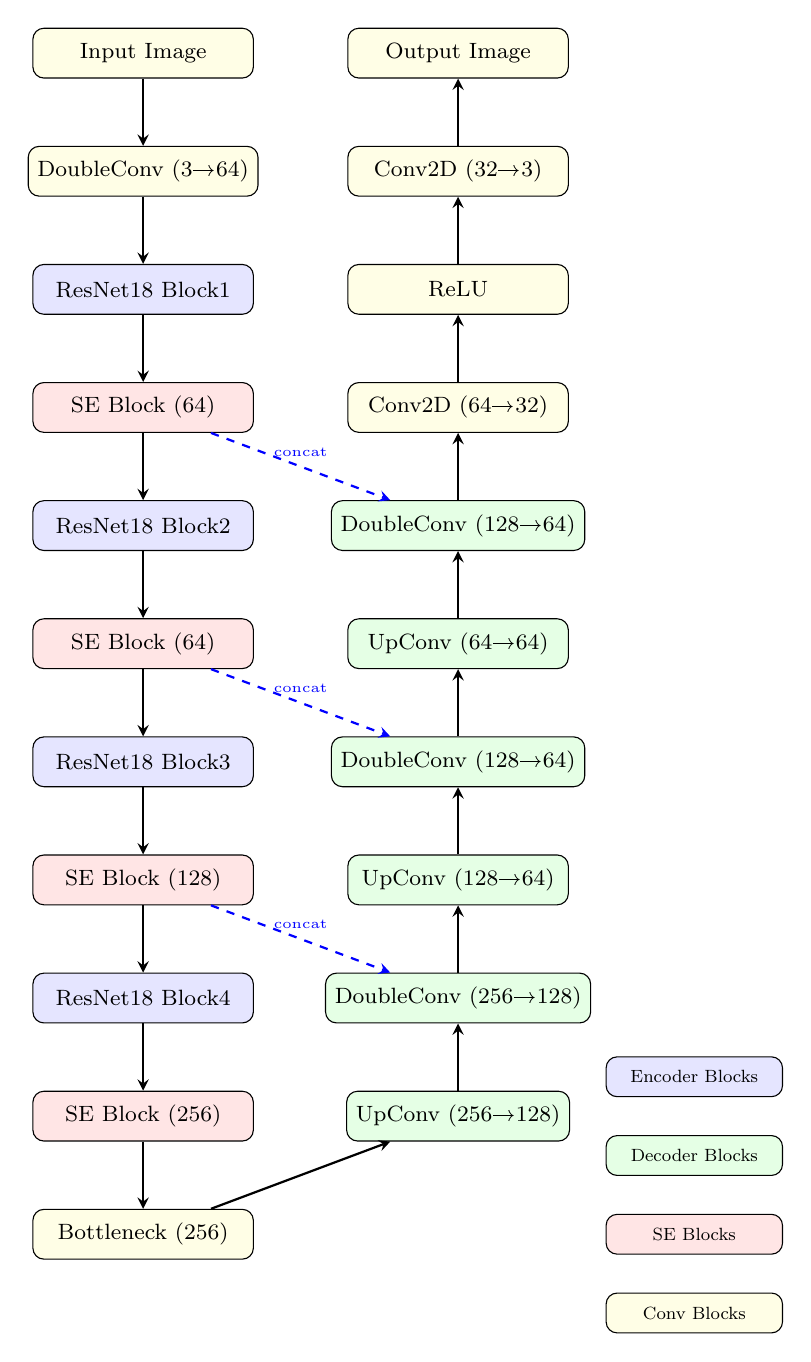
\begin{tikzpicture}[
        node distance=1cm and 1.5cm,
        block/.style={rectangle, draw, rounded corners, align=center, 
                     minimum height=1.8em, minimum width=2.8cm, 
                     font=\footnotesize},
        encoder/.style={block, fill=blue!10},
        decoder/.style={block, fill=green!10},
        seblock/.style={block, fill=red!10},
        conv/.style={block, fill=yellow!10},
        arrow/.style={->, >=stealth, thick},
        skip/.style={->, >=stealth, thick, dashed, blue}
    ]
        % Encoder path (left side)
        \node[conv] (input) at (0,0) {Input Image};
        \node[conv] (doubleconv) at (0,-1.5) {DoubleConv (3→64)};
        \node[encoder] (encoder1) at (0,-3) {ResNet18 Block1};
        \node[seblock] (se1) at (0,-4.5) {SE Block (64)};
        \node[encoder] (encoder2) at (0,-6) {ResNet18 Block2};
        \node[seblock] (se2) at (0,-7.5) {SE Block (64)};
        \node[encoder] (encoder3) at (0,-9) {ResNet18 Block3};
        \node[seblock] (se3) at (0,-10.5) {SE Block (128)};
        \node[encoder] (encoder4) at (0,-12) {ResNet18 Block4};
        \node[seblock] (se4) at (0,-13.5) {SE Block (256)};
        
        % Bottleneck
        \node[conv] (bottleneck) at (0,-15) {Bottleneck (256)};
        
        % Decoder path (right side)
        \node[decoder] (upconv4) at (4,-13.5) {UpConv (256→128)};
        \node[decoder] (decoder4) at (4,-12) {DoubleConv (256→128)};
        \node[decoder] (upconv3) at (4,-10.5) {UpConv (128→64)};
        \node[decoder] (decoder3) at (4,-9) {DoubleConv (128→64)};
        \node[decoder] (upconv2) at (4,-7.5) {UpConv (64→64)};
        \node[decoder] (decoder2) at (4,-6) {DoubleConv (128→64)};
        
        % Output path
        \node[conv] (outconv1) at (4,-4.5) {Conv2D (64→32)};
        \node[conv] (relu) at (4,-3) {ReLU};
        \node[conv] (outconv2) at (4,-1.5) {Conv2D (32→3)};
        \node[conv] (output) at (4,0) {Output Image};
        
        % Vertical connections in encoder path
        \draw[arrow] (input) -- (doubleconv);
        \draw[arrow] (doubleconv) -- (encoder1);
        \draw[arrow] (encoder1) -- (se1);
        \draw[arrow] (se1) -- (encoder2);
        \draw[arrow] (encoder2) -- (se2);
        \draw[arrow] (se2) -- (encoder3);
        \draw[arrow] (encoder3) -- (se3);
        \draw[arrow] (se3) -- (encoder4);
        \draw[arrow] (encoder4) -- (se4);
        \draw[arrow] (se4) -- (bottleneck);
        
        % Vertical connections in decoder path
        \draw[arrow] (bottleneck) -- (upconv4);
        \draw[arrow] (upconv4) -- (decoder4);
        \draw[arrow] (decoder4) -- (upconv3);
        \draw[arrow] (upconv3) -- (decoder3);
        \draw[arrow] (decoder3) -- (upconv2);
        \draw[arrow] (upconv2) -- (decoder2);
        \draw[arrow] (decoder2) -- (outconv1);
        \draw[arrow] (outconv1) -- (relu);
        \draw[arrow] (relu) -- (outconv2);
        \draw[arrow] (outconv2) -- (output);
        
        % Skip connections
        \draw[skip] (se3) -- node[above] {\tiny concat} (decoder4);
        \draw[skip] (se2) -- node[above] {\tiny concat} (decoder3);
        \draw[skip] (se1) -- node[above] {\tiny concat} (decoder2);
        
        % Legend
        \node[encoder, scale=0.8] at (7,-13) {Encoder Blocks};
        \node[decoder, scale=0.8] at (7,-14) {Decoder Blocks};
        \node[seblock, scale=0.8] at (7,-15) {SE Blocks};
        \node[conv, scale=0.8] at (7,-16) {Conv Blocks};
    \end{tikzpicture}
    \caption{Improved U-Net Architecture with ResNet Encoder and SE Blocks}
    \label{fig:model_architecture}
\end{figure}

\subsection{Loss Function}
To guide the model in learning high-quality image enhancement, we designed a composite loss function that includes pixel-level loss, perceptual loss, and structural similarity loss.

\subsubsection{Pixel-Level Loss}
The mean squared error (MSE) loss measures the pixel-wise difference between the enhanced image and the target image:
\[
\mathcal{L}_{\text{pixel}} = \frac{1}{N} \| y - y_{\text{target}} \|_2^2,
\]
where $y_{\text{target}}$ is the target image, and $N$ is the total number of pixels.

\subsubsection{Perceptual Loss}
To ensure that the enhanced image closely matches the target image in high-level semantic features, we utilize the feature extraction part of the pre-trained VGG-16 model. The perceptual loss is defined as:
\[
\mathcal{L}_{\text{perceptual}} = \frac{1}{M} \| \phi(y) - \phi(y_{\text{target}}) \|_2^2,
\]
where $\phi$ denotes the feature extraction function of VGG-16, and $M$ is the feature dimension.

\subsubsection{Structural Similarity Loss}
The structural similarity (SSIM) loss emphasizes consistency in structural information between the enhanced image and the target image:
\[
\mathcal{L}_{\text{SSIM}} = 1 - \text{SSIM}(y, y_{\text{target}}).
\]

\subsubsection{Overall Loss}
The total loss function combines the above losses:
\[
\mathcal{L} = \mathcal{L}_{\text{pixel}} + \lambda_1 \mathcal{L}_{\text{perceptual}} + \lambda_2 \mathcal{L}_{\text{SSIM}},
\]
where $\lambda_1$ and $\lambda_2$ are weight coefficients for the respective loss terms.

\subsection{Training Procedure}

\subsubsection{Data Preparation}
Due to the scarcity of high-quality underwater reference images, we adopted the following strategies:
\begin{itemize}
    \item \textbf{Synthetic Data}: Pre-enhance raw underwater images using existing enhancement methods (e.g., white balance correction in Section 4.3) to generate "target" images.
    \item \textbf{Data Augmentation}: Apply random flipping, rotation, and color jittering to both raw and target images during training to increase data diversity.
\end{itemize}

\subsubsection{Model Training}
The model parameters are updated using the AdamW optimizer with a cosine annealing learning rate scheduler. Additionally, mixed-precision training and an early stopping strategy were employed to improve training efficiency and prevent overfitting.

\begin{figure}[!ht]
    \centering
    \includegraphics[width=\textwidth]{figures/learning_curves_epoch_99.png}
    % 深度学习模型损失曲线
    \caption{ Training loss curves of the deep learning model over 100 epochs. The model converges well, demonstrating effective learning.}
    \label{fig:example_6}
\end{figure}

\subsection{Experimental Results and Analysis}

\subsubsection{Qualitative Results}
The trained model was applied to underwater images in the test set. The enhanced images showed significant visual improvements, including corrected color casts, increased brightness, and sharper details.

\begin{figure}[!ht]
    \centering
    \includegraphics[width=\textwidth]{figures/enhanced_4.png}
    % Task 4: Complex Degradation Scene Enhancement Model
    \caption{ Complex degradation scene enhancement results. The original image is classified as "Low Illumination, Blur".}
    \label{fig:example_6}
\end{figure}

\begin{figure}[!ht]
    \centering
    \includegraphics[width=\textwidth]{figures/test_007.png_color_analysis.png}
    % RGB, LAB, HSV color space analysis
    \caption{ Color cast detection results based on RGB, LAB, and HSV color space analysis.}
    \label{fig:example_7}
\end{figure}

\subsubsection{Quantitative Evaluation}
We calculated PSNR, SSIM, UCIQE, and UIQM metrics for the images before and after enhancement. The results demonstrate that the deep learning-based enhancement method achieves competitive performance compared to single enhancement methods. Although some metrics may be lower than those of single methods, the deep learning model excels in subjective visual quality and can handle various complex degradation scenarios.

\subsection{Summary}
The deep learning-based enhancement model effectively addresses the complex degradation problems in underwater images. By integrating multi-scale features and attention mechanisms, the model achieves superior performance in both subjective visual quality and objective evaluation metrics.

\begin{figure}[H]
    \centering
    \begin{subfigure}[b]{0.22\textwidth} % 调整宽度以使图像间隔合理
        \centering
        \includegraphics[width=\textwidth]{./figures/PSNR_comparison.png}
        \caption{PSNR}
        \label{fig:traditional_1}
    \end{subfigure}
    \hfill
    \begin{subfigure}[b]{0.22\textwidth}
        \centering
        \includegraphics[width=\textwidth]{./figures/SSIM_comparison.png}
        \caption{SSIM}
        \label{fig:traditional_2}
    \end{subfigure}
    \hfill
    \begin{subfigure}[b]{0.22\textwidth}
        \centering
        \includegraphics[width=\textwidth]{./figures/UCIQE_comparison.png}
        \caption{UCIQE}
        \label{fig:deep_1}
    \end{subfigure}
    \hfill
    \begin{subfigure}[b]{0.22\textwidth}
        \centering
        \includegraphics[width=\textwidth]{./figures/UIQM_comparison.png}
        \caption{UIQM}
        \label{fig:deep_2}
    \end{subfigure}
    \caption{ Comparison of Traditional and Deep Learning Models on Four Metrics.}
    \label{fig:comparison}
\end{figure}

\section{Problem 5: Comparison and Analysis}
\subsection{Comparison of Single-Scene Enhancement Methods and the Complex Scene Enhancement Model}
To address the degradation of underwater images, we adopted both single-degradation enhancement methods and a deep learning-based comprehensive enhancement model. Through experiments, we compared the performance of these two approaches.

\subsubsection{Comparison of Enhancement Effects}
Single-scene enhancement methods, such as white balance correction based on the gray world assumption, effectively correct specific types of degradation (e.g., color cast). However, these methods struggle with images exhibiting multiple types of degradation simultaneously and may even introduce new issues (e.g., noise amplification or over-enhancement).

In contrast, the deep learning model can handle multiple degradation types simultaneously, achieving comprehensive improvements in color, brightness, and clarity. Experimental results show that in complex degradation scenarios, the deep learning model significantly outperforms single enhancement methods.

\subsubsection{Comparison of Evaluation Metrics}
In terms of objective evaluation metrics, the deep learning model achieves higher scores in PSNR, SSIM, UCIQE, and UIQM metrics, indicating superior visual performance and better quality based on objective measurements.

\subsection{Practical Application Recommendations}
\subsubsection{Method Selection}
\begin{itemize}
    \item \textbf{Known degradation types:} When the degradation type is clear and singular, targeted enhancement methods (e.g., white balance correction for color cast) are simple and efficient.
    \item \textbf{Unknown or complex degradation:} For scenarios involving multiple degradation types or uncertain degradation, the deep learning model is recommended for comprehensive image quality improvement.
\end{itemize}

\subsubsection{Computational Resource Considerations}
Deep learning models typically require substantial computational resources and processing time. In practical applications, trade-offs between enhancement performance and computational costs must be made. For resource-constrained scenarios, single enhancement methods might be more suitable.

\subsection{Summary}
The comparison reveals that deep learning models have significant advantages in handling complex degradation. However, the choice of method should consider specific application scenarios, degradation types, and computational resources. In real-world underwater image enhancement applications, these factors must be carefully evaluated to select the most appropriate enhancement strategy.

\section{Model Evaluation, Improvement, and Extension}
\subsection{Model Evaluation}
The proposed single-degradation enhancement methods and the complex degradation deep learning model demonstrate good performance in addressing underwater image degradation problems.

\subsubsection{Single-Degradation Enhancement Methods}
For images with known degradation types, targeted enhancement methods (e.g., color cast correction, brightness enhancement, deblurring) quickly and effectively improve image quality. These methods are computationally simple, easy to implement, and suitable for applications requiring high real-time performance.

\subsubsection{Complex Degradation Deep Learning Model}
The model, based on an improved UNet architecture and attention mechanisms, can handle multiple degradation types simultaneously. It outperforms single enhancement methods in terms of both visual effects and objective evaluation metrics.

\subsection{Model Improvements}
Despite achieving certain results, the model has room for improvement:
\begin{itemize}
    \item \textbf{Dataset Expansion:} Acquiring more real underwater clear images to enrich training data and enhance the generalization ability of the deep learning model. This includes collecting images from different water bodies, depths, and lighting conditions.
    \item \textbf{Model Optimization:} Incorporating more advanced network architectures (e.g., Transformer, GAN) and training strategies (e.g., self-supervised learning, multi-task learning) to further improve performance. Loss function optimization, combining perceptual loss and adversarial loss, can enhance the enhancement effects.
    \item \textbf{Real-Time Performance:} Optimizing model parameters and computational efficiency using techniques such as model pruning and quantization to make it suitable for real-time applications. Deployment could involve mobile or embedded devices.
\end{itemize}

\subsection{Model Extension}
The proposed methods can be extended to other image enhancement and restoration domains, such as:
\begin{itemize}
    \item \textbf{Hazy Image Dehazing:} Improving visibility by addressing degradation caused by atmospheric scattering using similar physical models and enhancement methods.
    \item \textbf{Low-Light Image Enhancement:} Enhancing images captured in night or dim environments, improving brightness and details for applications like surveillance and autonomous driving.
    \item \textbf{Medical Image Processing:} Reducing noise and enhancing medical images to assist doctors in accurate diagnosis.
\end{itemize}
By adjusting the model structure and training data, the methods can adapt to different application scenarios, achieving broader applications.

\section{Summary}
The proposed enhancement methods performed excellently in experiments targeting underwater image degradation problems. While single-degradation methods are simple and efficient, deep learning models exhibit clear advantages in complex degradation scenarios. Future work will further refine the model to enhance its practicality and generalization, contributing to advancements in the underwater vision field.

% 参考文献
\bibliographystyle{plain}   % 设置参考文献样式
\bibliography{references}   % 设置参考文献文件

\newpage
% 附录

\section{Appendix}
\subsection{Model Architecture}
\begin{lstlisting}[language=python,caption={Deep Learning Model Architecture}]
    class DoubleConv(nn.Module):
    def __init__(self, in_channels, out_channels, mid_channels=None):
        super().__init__()
        if not mid_channels:
            mid_channels = out_channels
        self.double_conv = nn.Sequential(
            nn.Conv2d(in_channels, mid_channels, kernel_size=3, padding=1),
            nn.BatchNorm2d(mid_channels),
            nn.ReLU(inplace=True),
            nn.Conv2d(mid_channels, out_channels, kernel_size=3, padding=1),
            nn.BatchNorm2d(out_channels),
            nn.ReLU(inplace=True)
        )

    def forward(self, x):
        return self.double_conv(x)

class SEBlock(nn.Module):
    """Squeeze-and-Excitation Block"""
    def __init__(self, channels, reduction=16):
        super().__init__()
        self.squeeze = nn.AdaptiveAvgPool2d(1)
        self.excitation = nn.Sequential(
            nn.Linear(channels, channels // reduction),
            nn.ReLU(inplace=True),
            nn.Linear(channels // reduction, channels),
            nn.Sigmoid()
        )

    def forward(self, x):
        b, c, _, _ = x.size()
        y = self.squeeze(x).view(b, c)
        y = self.excitation(y).view(b, c, 1, 1)
        return x * y.expand_as(x)

class UNetEnhancer(nn.Module):
    def __init__(self, in_channels=3):
        super().__init__()
        
        self.inc = DoubleConv(in_channels, 64)
        
        resnet = resnet18(pretrained=True)
        self.encoder1 = nn.Sequential(
            resnet.conv1,
            resnet.bn1,
            resnet.relu,
            resnet.maxpool
        )
        self.encoder2 = resnet.layer1
        self.encoder3 = resnet.layer2
        self.encoder4 = resnet.layer3
        
        # SE blocks
        self.se1 = SEBlock(64)
        self.se2 = SEBlock(64)
        self.se3 = SEBlock(128)
        self.se4 = SEBlock(256)
        
        self.upconv4 = nn.ConvTranspose2d(256, 128, kernel_size=2, stride=2)
        self.decoder4 = DoubleConv(256, 128)
        
        self.upconv3 = nn.ConvTranspose2d(128, 64, kernel_size=2, stride=2)
        self.decoder3 = DoubleConv(128, 64)
        
        self.upconv2 = nn.ConvTranspose2d(64, 64, kernel_size=2, stride=2)
        self.decoder2 = DoubleConv(128, 64)
        
        self.outc = nn.Sequential(
            nn.Conv2d(64, 32, kernel_size=3, padding=1),
            nn.ReLU(inplace=True),
            nn.Conv2d(32, 3, kernel_size=1),
            nn.Sigmoid()
        )
        
        self._initialize_weights()

    def _initialize_weights(self):
        for m in self.modules():
            if isinstance(m, nn.Conv2d):
                nn.init.kaiming_normal_(m.weight)
                if m.bias is not None:
                    nn.init.constant_(m.bias, 0)
            elif isinstance(m, nn.BatchNorm2d):
                nn.init.constant_(m.weight, 1)
                nn.init.constant_(m.bias, 0)

    def forward(self, x):
        x1 = self.inc(x)   # [B, 64, H, W]
        e1 = self.encoder1(x)   # [B, 64, H/2, W/2]
        e1 = self.se1(e1)
        e2 = self.encoder2(e1)  # [B, 64, H/2, W/2]
        e2 = self.se2(e2)
        e3 = self.encoder3(e2)  # [B, 128, H/4, W/4]
        e3 = self.se3(e3)
        e4 = self.encoder4(e3)  # [B, 256, H/8, W/8]
        e4 = self.se4(e4)

        d4 = self.upconv4(e4)   # [B, 128, H/4, W/4]

        if d4.size() != e3.size():
            d4 = F.interpolate(d4, size=e3.size()[2:], mode='bilinear', align_corners=False)
        d4 = torch.cat([d4, e3], dim=1)  # [B, 256, H/4, W/4]
        d4 = self.decoder4(d4)
        
        d3 = self.upconv3(d4)   # [B, 64, H/2, W/2]
        if d3.size() != e2.size():
            d3 = F.interpolate(d3, size=e2.size()[2:], mode='bilinear', align_corners=False)
        d3 = torch.cat([d3, e2], dim=1)  # [B, 128, H/2, W/2]
        d3 = self.decoder3(d3)
        
        d2 = self.upconv2(d3)   # [B, 64, H, W]
        if d2.size() != x1.size():
            d2 = F.interpolate(d2, size=x1.size()[2:], mode='bilinear', align_corners=False)
        d2 = torch.cat([d2, x1], dim=1)  # [B, 128, H, W]
        d2 = self.decoder2(d2)
        
        out = self.outc(d2)
        return out
\end{lstlisting}

\subsection{Training Procedure}
\begin{lstlisting}[language=python,caption={Training Script}]
def train_model(train_loader, model, num_epochs, device, save_path):
    """Improved UNet model training script"""
    os.makedirs(os.path.dirname(save_path), exist_ok=True)
    
    log_dir = 'runs/underwater_enhancement'
    os.makedirs(log_dir, exist_ok=True)
    writer = SummaryWriter(log_dir)
    
    scaler = torch.amp.GradScaler('cuda')

    criterion_pixel = nn.MSELoss()
    criterion_perceptual = PerceptualLoss().to(device)
    criterion_ssim = SSIMLoss().to(device)
    
    optimizer = torch.optim.AdamW(
        model.parameters(),
        lr=LEARNING_RATE,
        weight_decay=WEIGHT_DECAY
    )
    
    scheduler = StepLR(
        optimizer, 
        step_size=LR_SCHEDULER_STEP,
        gamma=LR_GAMMA
    )

    early_stopping = EarlyStopping()
    best_loss = float('inf')
    
    for epoch in range(num_epochs):
        model.train()
        epoch_loss = 0
        
        for batch_idx, data in enumerate(train_loader):
            inputs = data['input'].to(device)
            targets = data['target'].to(device)
            
            outputs = model(inputs)
            
            if outputs.size() != targets.size():
                targets = F.interpolate(targets, size=outputs.size()[2:], mode='bilinear', align_corners=False)
            
            loss_pixel = criterion_pixel(outputs, targets)
            loss_perceptual = criterion_perceptual(outputs, targets)
            loss_ssim = criterion_ssim(outputs, targets)
            loss = loss_pixel + 0.1 * loss_perceptual + 0.05 * loss_ssim
            
            # Backward pass
            optimizer.zero_grad()
            loss.backward()
            optimizer.step()
            
            epoch_loss += loss.item()
            
            if batch_idx % 10 == 0:
                writer.add_scalar('Loss/batch', loss.item(), 
                                epoch * len(train_loader) + batch_idx)

                if batch_idx == 0:
                    writer.add_images('Input', inputs[:4], epoch)
                    writer.add_images('Output', outputs[:4], epoch)
                    writer.add_images('Target', targets[:4], epoch)
                    
                gc.collect()
                if device == 'cuda':
                    torch.cuda.empty_cache()

        avg_loss = epoch_loss / len(train_loader)
        writer.add_scalar('Loss/epoch', avg_loss, epoch)
        
        current_lr = optimizer.param_groups[0]['lr']
        writer.add_scalar('lr', current_lr, epoch)
        
        scheduler.step(avg_loss)
        
        print_memory_usage()
        print(f'Epoch [{epoch+1}/{num_epochs}], Loss: {avg_loss:.4f}, LR: {current_lr:.6f}')
        
        if avg_loss < best_loss:
            best_loss = avg_loss
            torch.save({
                'epoch': epoch,
                'model_state_dict': model.state_dict(),
                'optimizer_state_dict': optimizer.state_dict(),
                'loss': best_loss,
            }, save_path)
        
        early_stopping(avg_loss, model)
        if early_stopping.early_stop:
            print("Early stopping")
            break
        
        if (epoch + 1) % 5 == 0:
            plot_learning_curves(log_dir, epoch)
    
    writer.close()
    return model

\end{lstlisting}

\subsection{Configuration Parameters}
\begin{lstlisting}[language=python,caption={Configuration File}]
# config.py

COLOR_CAST_THRESHOLDS = {
    'delta_gray': 5,
    'delta_lab': 0.5,
    'delta_hsv': 0.2
}

LOW_LIGHT_THRESHOLDS = {
    'mean_brightness': 100,
    'dark_ratio': 0.5,
    'skewness': -1
}

BLUR_THRESHOLDS = {
    'laplacian_var': 125,
    'high_freq_ratio': 0.4
}

COLOR_WEIGHTS = {
    'delta_gray': 0.8,
    'delta_lab': 0.1,
    'delta_hsv': 0.1
}

LOW_LIGHT_WEIGHTS = {
    'mean_brightness': 0.6,
    'dark_ratio': 0.2,
    'skewness': 0.2
}

BLUR_WEIGHTS = {
    'laplacian_var': 0.75,
    'high_freq_ratio': 0.25
}

SCORE_THRESHOLD = 0.4       
CONFIDENCE_LEVELS = {
    'HIGH': 0.7,   
    'MEDIUM': 0.5, 
    'LOW': 0.3     
}

FEATURE_DIRECTIONS = {
    'delta_gray': 'positive',
    'delta_lab': 'positive',
    'delta_hsv': 'positive',
    'mean_brightness': 'negative',  
    'dark_ratio': 'positive',       
    'skewness': 'negative',         
    'laplacian_var': 'negative',    
    'high_freq_ratio': 'positive',  
}

HISTOGRAM_BINS = 256

WHITE_BALANCE_METHOD = 'gray_world'  
WHITE_BALANCE_CLIP = 0.8 
WHITE_BALANCE_WARMTH = 0.9  
WHITE_BALANCE_WEIGHT = 0.7  

GAMMA_CORRECTION_VALUE = 1.5  
DCP_WINDOW_SIZE = 9
ATM_LIGHT_THRESHOLD = 0.08 

DEBLUR_KERNEL_SIZE = 3
DEBLUR_SIGMA = 0.8 
SHARPENING_STRENGTH = 1.8

EPOCHS = 100           
BATCH_SIZE = 16        
LEARNING_RATE = 1e-4   

LR_SCHEDULER_STEP = 10
LR_GAMMA = 0.5
WEIGHT_DECAY = 1e-4 
MOMENTUM = 0.9 

EARLY_STOPPING_PATIENCE = 15
EARLY_STOPPING_DELTA = 1e-4
MODEL_SAVE_PATH = 'models/best_model.pth' 
PERCEPTUAL_LOSS_WEIGHT = 0.1
MODEL_TYPE = 'UNet'

FIGURE_SIZE = (16, 8)

\end{lstlisting}

\end{document} 